\chapter{Applications}
\label{ch:applications}


\section{Areas of application}
\label{sect:app_areas}

	\subsection{Social networks}
	\label{ssect:social_networks}
	
	Social networks are today's natural candidates for graph based algorithms, as they have been rising to power and fame over the previous decade and a half. Of course most social graphs in use today are far too big for any client or server side application to handle, and are therefore only interesting to programmers and architects of database clusters, high performance grid-computing developers and data-center engineers. Because of this, I am going to confine myself to the topic of local sphere recommenders, where I believe small graph computing to be able to have some real world influence. In order to get to this point, we will first need to take a look at the shape and size of typical recommendation processes (themselves forming subgraphs of larger networks), which in the following section will be termed 'cascades'.
	
	\subsubsection{Network recommendation analysis}
	\label{sssect:net_rec_anal}
	
	\citet{RecCascades}, The recommender cascade paper...
	
	* in the present paper, we are able to observe the cascades but not the underlying social network
	* In our work we need to efficiently enumerate and count cascade subgraphs
	* most of the prior work in this area is focused on graphs that are richly
	labeled and undirected, often motivated by applications to chemical compound
	and bioinformatics datasets
	* subgraphs based purely on their structures
	* The first recipient to purchase the item received a discount, and the sender received a referral credit with monetary value. A person could make recommendations on a product only after purchasing it. Since each sender had an incentive for making effective referrals, it is natural to hypothesize that this dataset is a good source of cascades.
	* Recommendation network is not the same as the underlying social network structure; actually, only the recommendation network was considered in their analysis of cascades.
	* recommendation subgraphs of the different products (DVDs, books, etc.)
	* all networks are very sparsely linked
	* At the end of the two-year period, the largest connected component contained fewer than 2.5% of the nodes
	* Observe that for DVDs 9% of purchases are associated with a recommendation, for books 3%, music 1.5% and video less than 1%.
	* One might imagine cascades to be trees or near-trees. In fact, we find that recommendations create essentially arbitrary graphs: there can be multiple recommendations on the same product or multiple product recommendations between the same pair of nodes; there are multiple purchases of the same product by the same individual (this is natural given that many items are purchased as gifts); and one also finds many cycles.
	- Delete late recommendations
	- Delete all nodes that didn't purchase the product
	* Cascades form graphs, and it's necessary to figure out which cascades are similar to one another -> graph isomorphism problem
	- Why is similarity important? To figure out how many **types** of cascades exist.
	- No *polynomial-time* algorithm is known for the graph isomorphism problem
	- Heuristic approximation via a graph **signature**
	- nr. of nodes
	- nr. of edges
	- sorted in- and out-degrees (degree distribution?)
	- graphs less than 9 nodes: exact matching
	- graphs < 500 nodes: also include the singular values of the adjacency matrix (via singular value decomposition)
	- a small minority of cascades are larger than 9 nodes
	* Results:
	- For books the largest cascade has 95 nodes and 231 edges. For DVDs the largest cascade is eight times larger (n = 791, e = 5544). The cascades involving music or videos are much smaller; the largest cascades are n = 13, e = 56 and n = 37, e = 169 respectively
	- For DVDs, the log fit function of cascade size to count is similar to books and music for smaller sized cascades, and exhibit unique behavior for larger cascades, which in this experiments were only found for the DVD category.
	- the number of purchases decaying as a function of rank faster than the number of recommendations does
	- **Make table**: For books we identified 122,657 cascades, of which 959 are topologically different. There are 213 cascades that occur at least ten times. For DVDs we identified 289,055 cascades, 87,614 are topologically different, and 3,015 cascades occur at least ten times. For music we identified 13,330 cascades, 158 were topologically different, and only 23 cascades occurred at least ten times. Videos were the least rich, with 1,928 subgraphs containing 109 unique patterns, and only 12 subgraphs occurring at least ten times.
	- Splits are more frequent than collisions
	* Conclusion:
	- Recommendations -> Complex social behavior
	- NOT ONLY STATISTICALLY WITH GENERAL NETWORK PROPERTIES
	- A concluding, general observation is that the frequency of cascade subgraphs does not simply decrease monotonically in the number of nodes and edges; for example, G5 is more frequent than either of its subgraphs G2 and G4 in DVDs and videos (and more frequent than G4 in books and music). Thus, frequency appears to reflect properties of the underlying social network (the clustering of people who know each other), as well as properties of the ways in which recommendations typically get made (e.g. splits are more common than collisions)
	
	\begin{figure}[ht]
		\label{fig_cascade_size_count}
		\begin{center}
			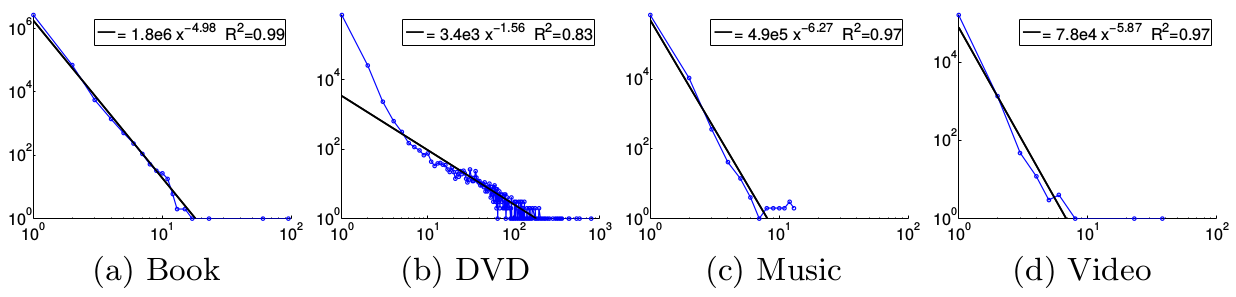
\includegraphics[width=1\textwidth]{figures/rec_cascades_size_count}
			\caption{Size distribution of recommendation cascades for four product types}
			\small
			This diagram was taken from \citep{RecCascades}, page 7.
		\end{center}
	\end{figure}
	
	
	\subsubsection{The local sphere (idea)}
	\label{sssect:the_local_sphere}
	
	The idea of a local sphere and computations applied to it comes from the author's (possibly incorrect, but natural) insight that the relevance of recommendations behaves as a function of network vicinity / node influence:
	
	\begin{itemize}
		\item Lets call the whole social graph and all interactions in it the 'global sphere'.
		\item Recommendations to users are then computed over the global sphere, which takes an amount of resources exponential to the size of the underlying graph.
		\item Let's further assume that 95\% of all relevant (accepted) recommendations in a social network like facebook are those that are derived from the immediate local neighborhood of a node (about 2 degrees..)
		\item Two degrees are also what Facebook allows programmers (as of 2013) to query via their graph API from any signed-on and authenticated user, apparently in an effort to prevent automatic traversal / exploration of their most valuable business asset.
		\item Let's call this immediate local neighborhood the 'local sphere'
	\end{itemize}
		
	Now let's also consider how modern publish/subscribe based frameworks (like Sails, Meteor, Hapi or Derby, only to mention some JavaScript libraries) handle data communication between server and client:
	
	\begin{itemize}
		\item The server offers some subscriptions on it's data, usually limiting access to items based on identity, authorization or user role provided by the client.
		\item The client defines some subscriptions on server-side data collections (tables), representing the client's wish for information regardless of it's status or authority.
		\item Publication as well as subscription can be seen as a mathematical subset of all the data in the database.
		\item An algorithm inside the respective framework resolves those (potentially conflicting) interests by computing the intersection set of the data provided / requested.
		\item The intersection data set is then pushed to the client (in our case the browser) as soon as it becomes available or is updated, which makes this model ideal for real-time interaction and communication between clients.
		\item The sum total of all the data pushed to the client is equivalent to the 'local sphere' we described earlier - HOWEVER - their inherent graph structure is lost during the transmission, so that the client can only see them as isolated fragments without context.
	\end{itemize}
	
	The combination of those two ideas now enables us to envision the following scenario:
	
	\begin{itemize}
		\item Instead of interpreting all data items in the local sphere as isolated entities, we retain their graph structure enabling the client to gain hitherto unachieved knowledge and insights into its already available data.
		\item We therefore need a graph library in the browser, not only to represent the local sphere graph, but also to analyze it in order to take intelligent actions that were previously reserved for the server-side (data center) infrastructure.
		\item No complex graph partitioning algorithm on the server is necessary, as we can use the natural set contraints inherent in any web application:
		\begin{itemize}
			\item e.g. in a social network, the client will have access to all its immediate friends, social activities and interest groups
			\item in a project management tool, the client naturally has access to the data of all team members, to-do lists, milestones, resources etc.
		\end{itemize}
		If our 95\%-relevance assumption mentioned earlier holds, we can achieve great scaling efficiency by introducing the local sphere concept:
		\begin{itemize}
			\item the client can immediately perform computations like recommendations on the subgraph of the local sphere.
			\item only recommendations accepted will have to be stored on the server (that is, cause additional network traffic).
			\item the client is easily able to recompute the relatively small local graphs in real-time, offering responsiveness far beyond today's best (server-side) infrastructures.
			\item as modern web frameworks transport all of the required data into the client store anyways, we do not add extra complexity to our servers and databases.
		\end{itemize}
		\item On the other hand, questions of data security / privacy will have to be dealt with, as we are talking about preemptively filling the client memory with possibly otherwise unnecessary or superfluous data.
	\end{itemize}
	
	
	\begin{figure}[ht]
		\label{fig_local_sphere}
		\begin{center}
			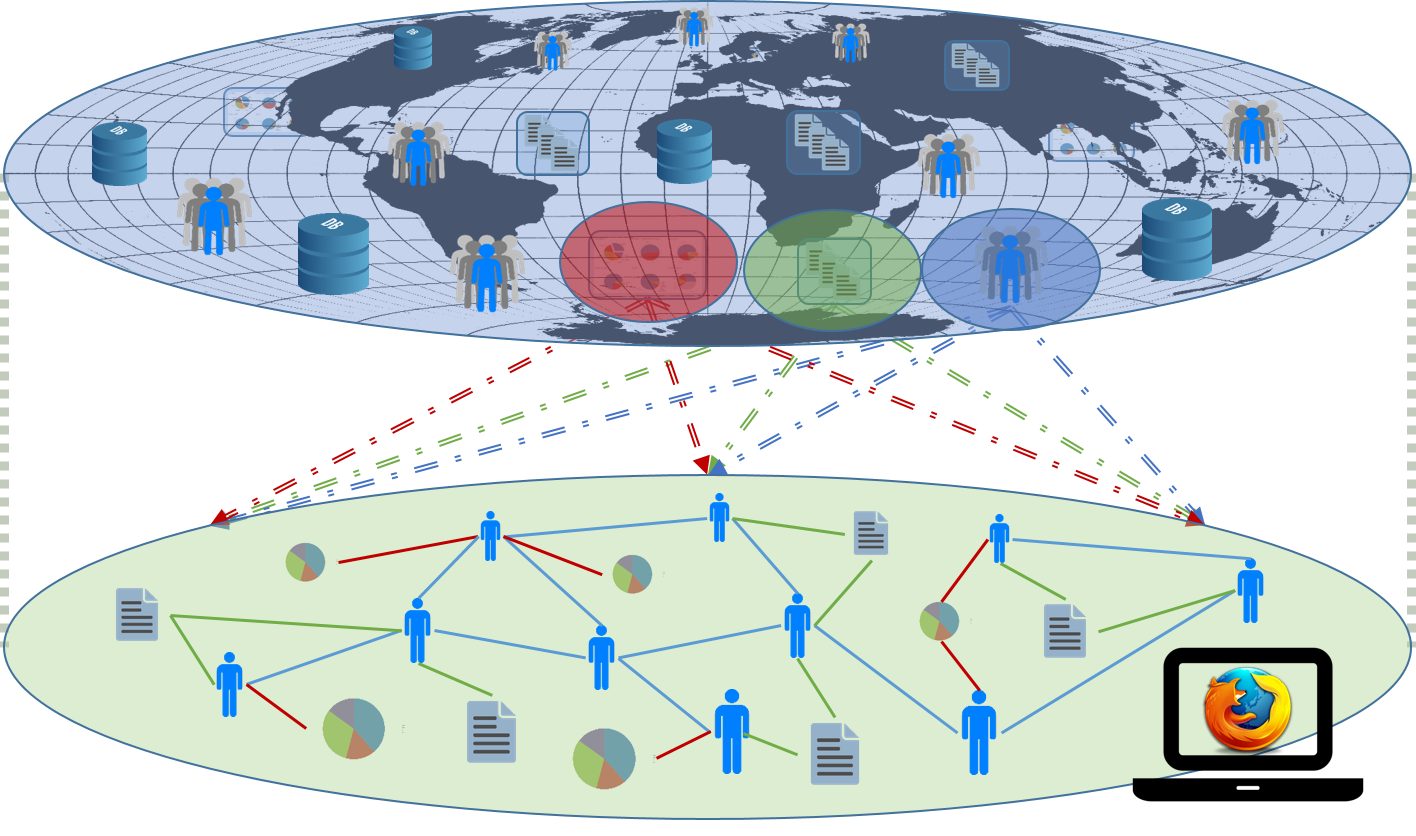
\includegraphics[width=1\textwidth]{figures/local_sphere}
			\caption{Local sphere projected from global sphere}
		\end{center}
		\small
		Only a very small portion of the global graph is actually visible from any connected client. The sum of all viewable items however, if properly conveyed to the client (i.e. with their connection information preserved), could form a subgraph of the whole network called the 'local sphere', which would allow the browser to utilize the underlying graph structure to extract hidden knowledge and perform graph computations on its own.
	\end{figure}
	
	
	Needless to say, GraphiniusJS would be an ideal candidate to explore this concept further and could, if used appropriately on carefully modeled local spheres, enable start-ups to compete with much larger companies employing complex and very expensive machine learning infrastructures.
	
	
	% \subsection{Communication networks}
	% \label{ssect:app_communication_networks}
	
	% \subsection{Transportation networks (Logistics)}
	% \label{ssect:app_transportation_networks}
	
	
	\subsection{Graph based image processing}
	\label{ssect:app_graph_img_proc}
	
	\begin{figure}[ht]
		\label{fig_graph_based_img_classification}
		\begin{center}
			
\includegraphics[width=1\textwidth]{figures/graph_img_class}
			\caption{Graph based image classification example}
		\end{center}
		\small
		1) a laser scan image of a nevus is oversegmented and 2) a graph extracted by interpreting region centroids as nodes and region adjacency as edges. 3) A belief propagation algorithm is applied to the resulting graph yielding 2) a converged state representing the nevus classification as benign or malignant.
	\end{figure}
	
	\subsection{Graph based NLP}
	\label{ssect:app_graph_nlp}
	
	\subsection{Biomedical applications (protein networks etc.)}
	\label{ssect:app_biomed}
	
	\subsection{Anonymization}
	\label{ssect:app_snonymization}
	
	\begin{figure}[ht]
		\label{fig_graph_based_img_classification}
		\begin{center}
			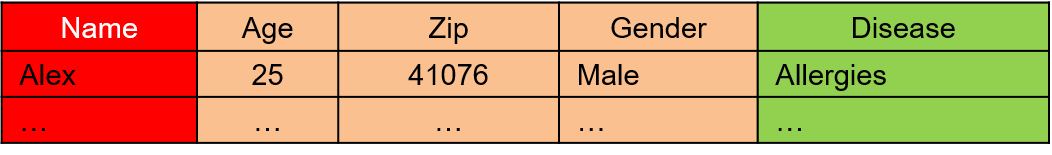
\includegraphics[width=0.9\textwidth]{figures/anonym/3typesofdata}
			\caption{The three types of data considered in (k-)anonymization}
		\end{center}
	\end{figure}
	
	
	\begin{figure}[H]
		\centering
		\begin{minipage}[b]{0.5\textwidth}
			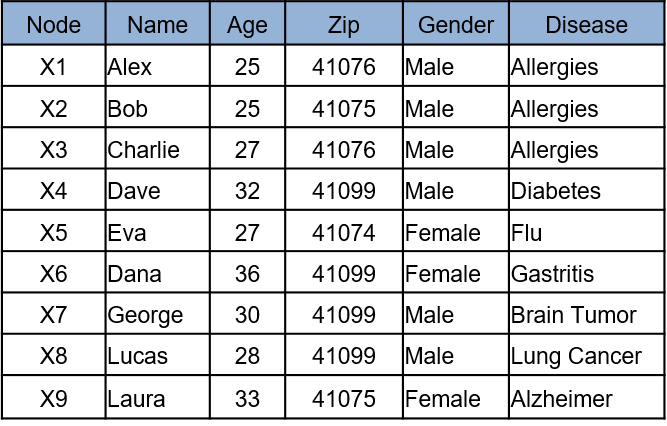
\includegraphics[width=\textwidth]{figures/anonym/k_anon_input}
		\end{minipage}
		\hfill
		\begin{minipage}[b]{0.418\textwidth}
			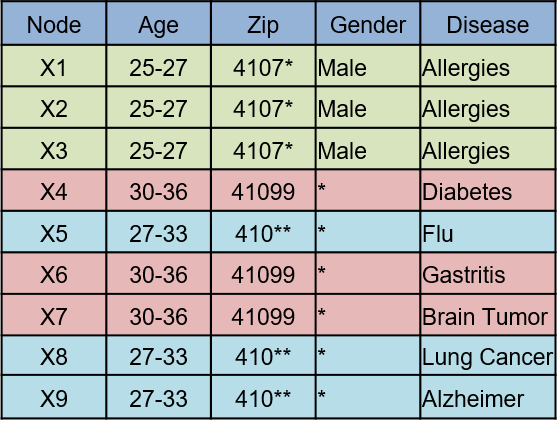
\includegraphics[width=\textwidth]{figures/anonym/k_anon_output}
		\end{minipage}
		\caption{Tabular anonymization: input table and anonymization result}
	\end{figure}	
	
	
	\subsection{Fraud detection}
	\label{ssect:fraud_detection}

	Polo chau's BP in MRF for spam classification work...

\section{Application specific requirements}
\label{section:app_requirements}

	\subsection{Data Structures}
	\label{ssect:data_gathering}
	
	\subsection{Data Cleaning}
	\label{ssect:data_cleaning}
	
	\subsection{Preprocessing}
	\label{ssect:preprocessing}
	
	Graph generation (ER model...)
	
	\subsection{Feature Selection}
	\label{ssect:feature_selection}
	
	\subsection{Data Mining}
	\label{ssect:data_mining}
	
	\subsection{Postprocessing}
	\label{ssect:postprocessing}
	
	\subsection{Visualization}
	\label{ssect:visualization}
	
	\subsection{Interaction / user feedback (iML)}
	\label{ssect:interaction}
	